% !TeX spellcheck = en_GB
\documentclass[12pt,fleqn,]{article}


\usepackage[english]{babel}
\usepackage{texfiles/SpeedyGonzales}
\usepackage{texfiles/MediocreMike}
\usepackage{multicol}
\usepackage{enumitem}
\usepackage{titlesec}
\usepackage{titling}
\titlespacing*{\section}{0pt}{0ex}{0ex}
\titlespacing{\subsection}{0pt}{1ex}{0ex}
\titlespacing{\subsubsection}{0pt}{0.5ex}{0ex}

\title{\vspace*{-3.75cm}Causal Inference on 7 Intertwined Effects \vspace*{-8mm}}
\author{\small Søren Holm, Oskar Wiese, Anders Henriksen and Anne Pedersen \\
\small {\texttt{\{s183911,s183917,s183904,s174300\}@student.dtu.dk}}}
\date{\vspace*{-3mm} \small \today}

\fancypagestyle{plain}
{
	\fancyhf{}
	\rfoot{Page \thepage{} of  \pageref{LastPage}}
	\renewcommand{\headrulewidth}{0pt}
}
\pagestyle{fancy}
\fancyhf{}
\lhead{Causal Inference}
\chead{}
\rhead{}
\rfoot{Page \thepage{} of \pageref{LastPage}}

\graphicspath{{imgs/}}
\linespread{1.15}


%TODO: \numberwithin{equation}{section}
%TODO: \numberwithin{footnote}{section}
%TODO: \numberwithin{figure}{section}
%TODO: \numberwithin{table}{section}


\begin{document}

\maketitle

\vspace*{-1cm}
\footnotesize\begin{abstract}
\scriptsize \noindent This project infers a causal model with as low cost as possible by querying points, using interventions and conditioning, and using statistically determined significant changes to find connections between nodes. After ten queries and one wrong guess, the causal model was found with a total cost of 725. The cost could have been lower if non-linear effects had been considered earlier.
\end{abstract}


\begin{multicols}{2}
	
	
\section{Introduction} 

Machine learning is great at the \textit{how}, but not at the \textit{why} of correlation. To mitigate this, intervention and conditioning can be used to infer the causal model at hand. In this project we infer a causal model as efficiently as possible. The purpose of the project is to achieve the lowest possible cost while determining the causal model. 

\section{Methods}
\texttt{Code available at \url{github.com/sorenmulli/active_learning_cases}} \newline
Before beginning the inference, an approach to the exploration/exploitation tradeoff to learning was chosen: This was, motivated by the cost parameters, to choose few data points, be more risk seeking and try to guess the causal system before full certainty.

To choose queries, an iterative process of constructing hypotheses consistent with the data at the given time was run. To choose the next query, the area of the graph where the hypotheses differed the most -- and the group disagreed the most -- was examined. Counterfactuals were (loosely) applied for each of the possible graphs before querying to have something to compare the query result to. 

To consider whether the change was 
\begin{itemize}
	\item Statistical tests: Student t test of means. Confidence interval on correlations. Comparing standard deviations. Bartlett's test of equal variance (nævner jeg i diskussionen)
	\item Visualization tools: Scatter plot of joint distribution. Comparisons of marginal distributions between queries.
	\item Writing up all 42 possible edges and eliminating the unlikely and achieving smaller set of possible edges where many are mutually exclusive given the following assumptions: The causal model is acyclic, which means that there are no cycles in the graph. The relationships between variables are linear, thus relationships can be revealed by correlations.
	\item .
\end{itemize}

%\textbf{First experiment:} 25 samples were drawn from the standard dataset. This shows some correlation between B and P, I and P, I and B and B and K.


%            I          P          S          B          K          A
%count  25.000000  25.000000  25.000000  25.000000  25.000000  25.000000
%mean    0.809233   0.737663   0.640000   0.608429   0.597139   1.083144
%std     1.182139   2.978524   0.489898   2.893580   0.169545   2.482438
%min    -2.005098  -6.655526   0.000000  -7.094593   0.271369  -3.700606
%25%     0.439067  -1.232216   0.000000  -0.829224   0.451194  -0.610884
%50%     1.003211   0.844233   1.000000   0.598850   0.600251   0.890359
%75%     1.285882   3.291850   1.000000   2.647563   0.691653   2.164174
%max     3.858524   5.468367   1.000000   5.714203   0.897285   5.826284

%       I         P         S         B         K         A
%I  1.000000  0.333897 -0.341654 -0.171798  0.291331  0.016965
%P  0.333897  1.000000 -0.106066  0.839574  0.414181  0.212517
%S -0.341654 -0.106066  1.000000  0.004534 -0.493877 -0.053259
%B -0.171798  0.839574  0.004534  1.000000  0.244270  0.132848
%K  0.291331  0.414181 -0.493877  0.244270  1.000000  0.079370
%A  0.016965  0.212517 -0.053259  0.132848  0.079370  1.000000


%\textbf{Second experiment:} Conditioning on S, since S is a categorical variable. S is conditioned to be 1. From this, we notice that the difference in the mean of K is significant. As such, K could be a child of S, since conditioning on S significantly changes the mean of K.
%s->k
%S has a slight change in the mean of I, so S could be parent of I.
%s->i

%p val for I mean: 0.08728710634129876
%p val I variance: 0.7074842288389503
%p val for P mean: 0.6201666892955116
%p val P variance: 0.8943920292984142
%p val for B mean: 0.9828623524458022
%p val B variance: 0.9765044743353757
%p val for K mean: 0.0060687195968801904
%p val K variance: 0.24180833861337936
%p val for A mean: 0.8102238966451225
%p val A variance: 0.6201097182165578


%\textbf{Third experiment:} 25 samples were drawn from the dataset with intervention on P=1. 
%The p-value from the t-test for testing significance of variance also shows that A has a significant difference after intervening on A, so A is probably a descendant of P. 
%p->a
%The same test on mean also shows that B is probably a descendant of P. 
%p->b
%I might also be a parent of B, since I and B got a big negative correlation after intervening on P.
%P and K seem correlated, so there could be a connection between these.
%k->p
%P could be a confounder between K and S, since their confounder is lowered after intervention on P.
%k<-p->s
%The correlation between I and B is higher than before intervention.
%i->b
%K and B are very correlated after the intervention.
%k->b


%            I     P          S          B          K          A
%count  25.000000  25.0  25.000000  25.000000  25.000000  25.000000
%mean    0.539471   1.0   0.720000   1.220529   0.591986   0.382593
%std     1.026998   0.0   0.458258   1.058383   0.192294   1.645327
%min    -1.165402   1.0   0.000000  -0.868669   0.263358  -3.771776
%25%    -0.185395   1.0   0.000000   0.551464   0.449007   0.091868
%50%     0.628475   1.0   1.000000   1.449233   0.613050   0.370300
%75%     0.993239   1.0   1.000000   2.138001   0.709600   1.522111
%max     2.868669   1.0   1.000000   2.966447   0.924464   2.979486

%          I   P         S         B         K         A
%I  1.000000 NaN  0.149217 -0.798053  0.371890  0.243146
%P       NaN NaN       NaN       NaN       NaN       NaN
%S  0.149217 NaN  1.000000  0.054516 -0.280234  0.266055
%B -0.798053 NaN  0.054516  1.000000 -0.468356 -0.213180
%K  0.371890 NaN -0.280234 -0.468356  1.000000 -0.149651
%A  0.243146 NaN  0.266055 -0.213180 -0.149651  1.000000
%
%p val for I mean: 0.3934156484682104
%p val I variance: 0.4958559471663381
%p val for S mean: 0.5537992160734111
%p val S variance: 0.7462341892822236
%p val for B mean: 0.32841672851104153
%p val B variance: 5.651184112058364e-06
%p val for K mean: 0.9203659378534125
%p val K variance: 0.5420753358523627
%p val for A mean: 0.24621510443236966
%p val A variance: 0.04915986030072988

%\textbf{Fourth experiment:} We sampled 50 points and intervened on K=1. Since intervention on K does not change P, it could be assumed that there is a confounder between P and K. This could be H.
%p<-h->k


%           I          P         S          B     K          A
%count  50.000000  50.000000  50.00000  50.000000  50.0  50.000000
%mean    0.952428   1.853977   0.70000   1.501549   1.0   0.852696
%std     0.904078   3.518374   0.46291   3.484149   0.0   3.236801
%min    -0.478087  -7.299935   0.00000  -7.328402   1.0  -9.617031
%25%     0.344298   0.062655   0.00000  -0.660957   1.0  -0.321875
%50%     0.892102   1.825095   1.00000   1.642826   1.0   1.086686
%75%     1.641766   4.317654   1.00000   3.774912   1.0   2.287807
%max     3.023864   8.983223   1.00000   9.380391   1.0  11.491141
%
%      I         P         S         B   K         A
%I  1.000000  0.213531 -0.140216 -0.103818 NaN  0.250387
%P  0.213531  1.000000 -0.142613  0.931324 NaN  0.012295
%S -0.140216 -0.142613  1.000000 -0.107631 NaN  0.185039
%B -0.103818  0.931324 -0.107631  1.000000 NaN -0.043386
%K       NaN       NaN       NaN       NaN NaN       NaN
%A  0.250387  0.012295  0.185039 -0.043386 NaN  1.000000
%
%p val for I mean: 0.5972710034477902
%p val I variance: 0.12141520656190993
%p val for B mean: 0.24487509163125104
%p val B variance: 0.3069268978956339
%p val for P mean: 0.1559487121326533
%p val P variance: 0.35826110265904465
%p val for S mean: 0.6130768858813082
%p val S variance: 0.7481530567819892
%p val for A mean: 0.7340946797325456
%p val A variance: 0.14890467211990585

%\textbf{Fifth experiment:} We sampled 50 datapoints, intervened on B=2 and conditioned on S=1. This would allow for us to show the true connection to K.
%
%\textbf{Sixth experiment: } Intervening on I=-2 with 50 samples. This makes the correlation of B and P become close to 1. This shows that I and P are the only parents of B.

\section{Results}

\subsubsection*{Queries}
\vspace*{-0.01cm}
\begin{enumerate}[]
	\item \(\mathcal D \in \RR^{25\times 6}\)
	\item \(\mathcal D \in \RR^{25\times 6}\quad \mathring{P\leftarrow1}\) 
	\item \(\mathcal D \in \RR^{50\times 6}\quad \mathring{K\leftarrow1}\) 
	\item \(\mathcal D \in \RR^{50\times 6}\quad \mathring{B\leftarrow1}\) 
	\item \(\mathcal D \in \RR^{50\times 6}\quad \mathring{I\leftarrow-2}\) 
	\item \(\mathcal D \in \RR^{50\times 6}\quad \mathring{I\leftarrow2}\ \wedge\ \mathring{P\leftarrow-2}\ \wedge\ \mathring{B\leftarrow-2}\)
	\item Wrong guess, see figure \ref{fig:wronggraph}

	\item \(\mathcal D \in \RR^{50\times 6}\quad  \mathring{A\leftarrow-1}\) 
	\item \(\mathcal D \in \RR^{75\times 6}\) 
	\item \(\mathcal D \in \RR^{50\times 6}\quad  \mathring{S\leftarrow1}\)
	\item \(\mathcal D \in \RR^{50\times 6}\quad  \mathring{B\leftarrow0}\) 
\end{enumerate}
\vspace*{-0.6cm}
\subsubsection*{Cost}
\[
\underbrace{475}_{\text{\# points}} + \underbrace {9}_ {\text{\# experiments}} \cdot 20 +\underbrace{70}_{\text{Guess}}=725
\]

\begin{figure}[H]
	\centering
	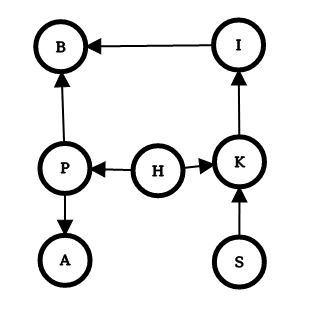
\includegraphics[width=.6\linewidth]{wronggraph}
	\caption{Wrong graph guess. Note that especially the effects on node A are misunderstood. Four edges are correct and three are wrong.}
	\label{fig:wronggraph}
\end{figure}
\begin{figure}[H]
	\centering
	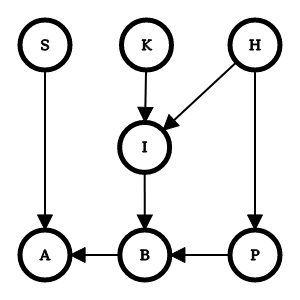
\includegraphics[width=.6\linewidth]{correctgraph}
	\caption{Correct graph. Amongst the corrections was K's reclassification from mediator to root cause.  }
	\label{fig:correctgraph}
\end{figure}

	
\section{Discussion}
The approach of a higher number of  queries, each with few data points, had strengths and weaknesses. This approach allowed for a healthy process of estimating the expected result under each of the hypotheses that were viable at that time and getting falsified these hypotheses often. 

It also had some drawbacks that resulted in some confusion. A large amount of time was spent trying to create complicated causal relationships to explain effects that the next query revealed to be spurious. This was amplified by most of the nodes having high variance compared to their numerical size.
% There were also issues with using statistical tests whose assumptions were questionable: Bartlett's test of equal variance gave false flags in the small data sets early on\footnote{The test is according to \cite{bartlett} sensitive to normality and suggested spuriously that }.

Another issue which held back the learning significantly and resulted in the need for at least one intervention on every variable was the underlying assumptions of the causal relationships. During most of the inference, linear, additive effects were the framework for modelling the graph. This misunderstanding resulted in some causal hypotheses to be overly complex to explain the effects on the node A. The effect from B to A was very difficult to encapsulate in the linear generative story and was thus often ignored and attributed to noise -- possibly an example of human confirmation bias. 

The non linear and more subtle effects were only discovered when (a) more data points were collected for the non-interventional data to iron out the spurious correlations, (b) the rigorous falsification of the 42 edges were performed and (c) \(\mathring{B\leftarrow0}\) was used to verify the suspicion of non linearity at A.
\\
\\
This task of finding the causal relationships from non-trivial data can be compared to the process of scientific discovery. While this causal graph is idealized and stripped of many practical problems of reality, the core goals and methods are comparable. The worries of where hidden, confounding variables, in this case H, lie in the network is a core issue.

A major difference to causal inference in real world data is that the number of possible explaining variables was fixed and known a priori in this project. A real study includes the challenge of limiting the included effects and may risk interpreting the results completely wrong if key variables are excluded. Even in this idealized setting, very similar problems occurred as key non-linear effects were missed, highlighting the pitfalls of considering a too small space of hypotheses. %Er version space dækkende for rummet af hypoteser?

\section{Learning outcomes} 
	
%	What new knowledge and skill you have gained.
%	What you think about the topics we have worked with.
%	What your own understanding is so far.
%	What you find puzzling, difficult, or contradictory.
%	What you need to know more about, and how you can find out.
%	What resources have helped you, that you might want to share. 
	
	By trying to explore and draw the causal model by making interventions on different variables, conditioning on the categorical variables and by looking at distributions, correlation, \textit{p}-values for student t-test and changes in variance, we have acquired a technique to infer causal relationships even for hidden variables. The difficulties in finding the causal relationships and determining the effects of the different variables have been discussed. However, in order to determine the causal graph, plotting and visualization tools have been very helpful along with the correlations displayed as well. 
	
\end{multicols}

\newpage
\begin{thebibliography}{9}
	

	
	
	

\end{thebibliography}


\appendix
\section{Visualizations}
\begin{figure}[H]
	\centering
	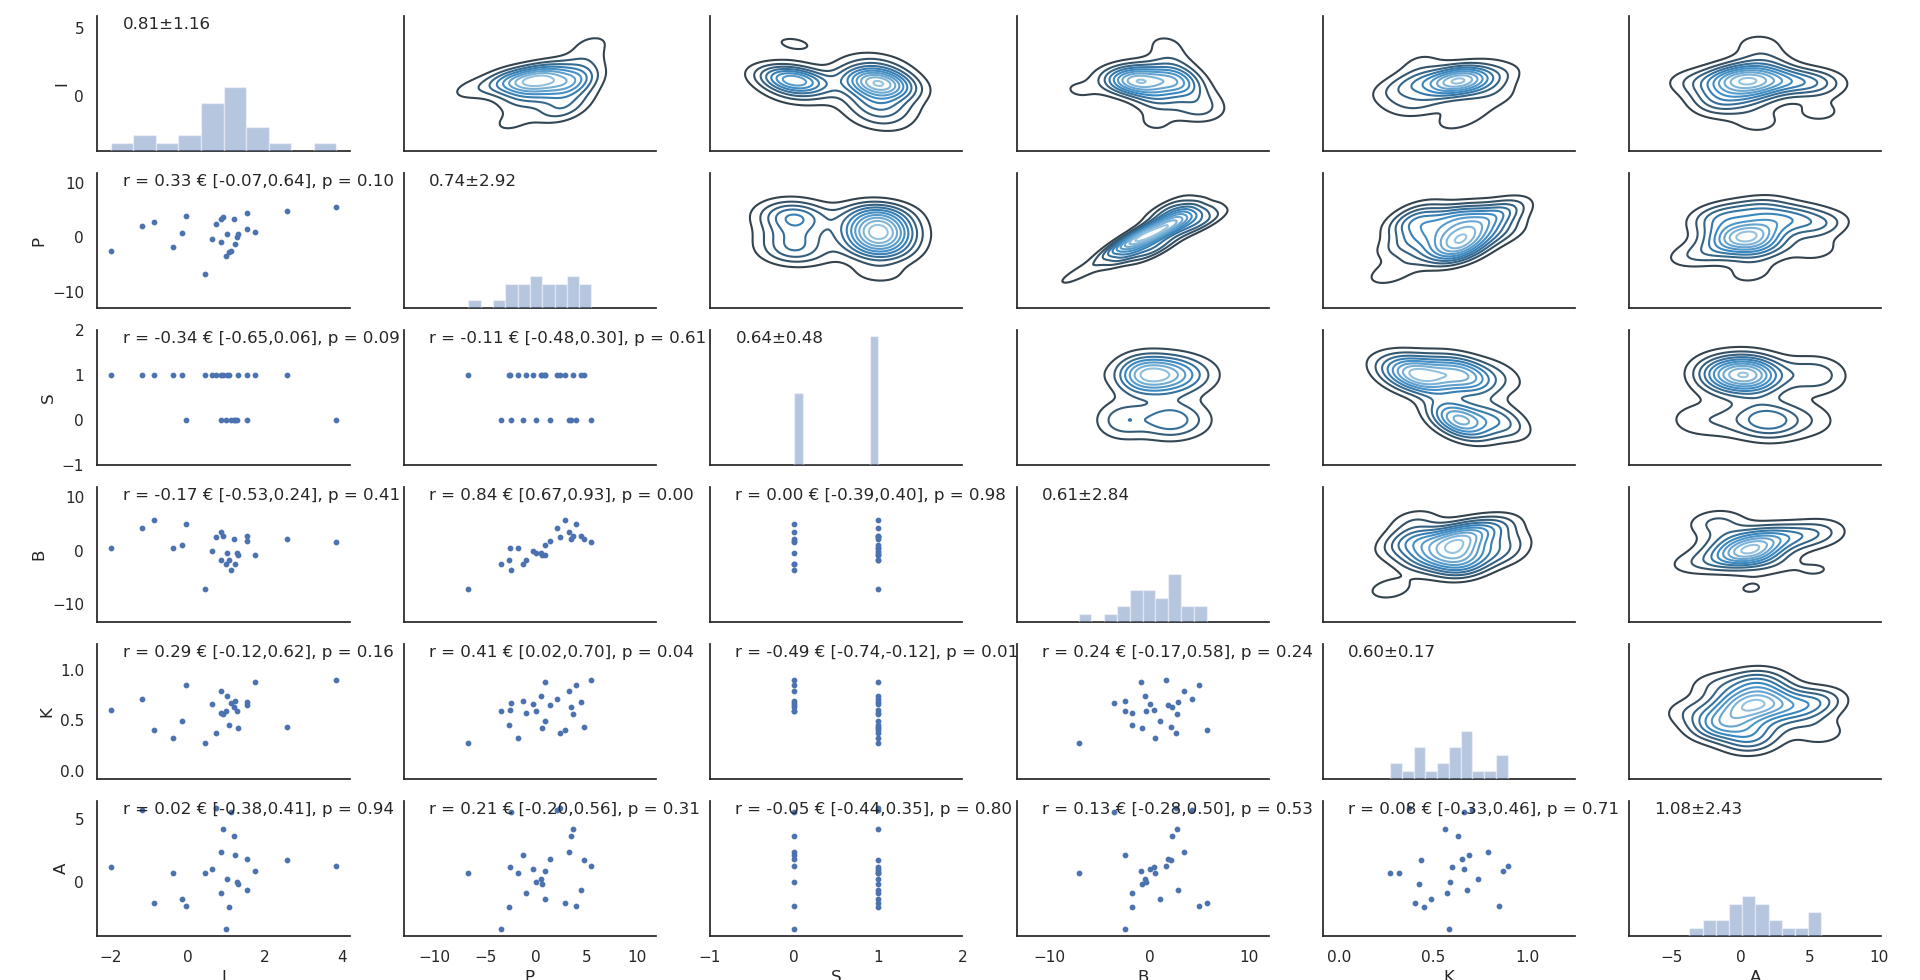
\includegraphics[width=\linewidth]{interNonedata}
	\caption{Visualization of the data set under no intervention}
	\label{fig:interNonedata}
\end{figure}
\begin{figure}[H]
	\centering
	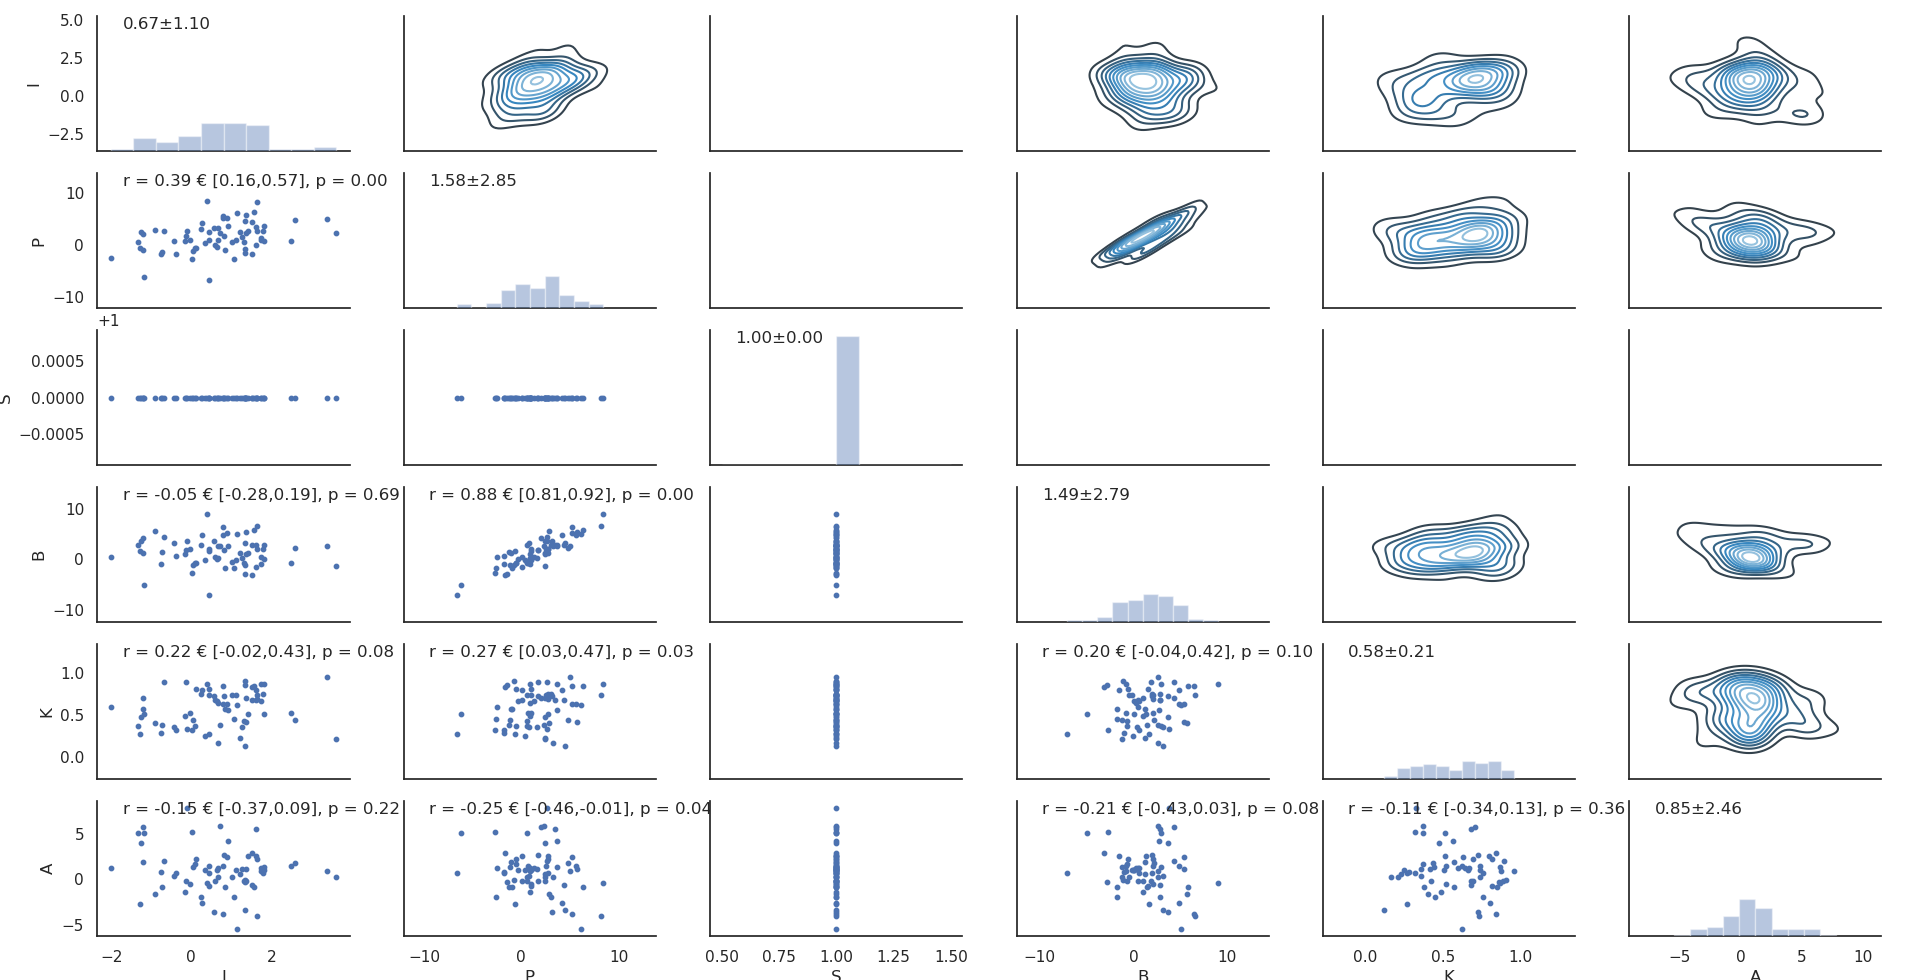
\includegraphics[width=\linewidth]{icondSdata}
	\caption{Visualization of the data set with S conditioned to 1}
	\label{fig:icondSdata}
\end{figure}
\begin{figure}[H]
	\centering
	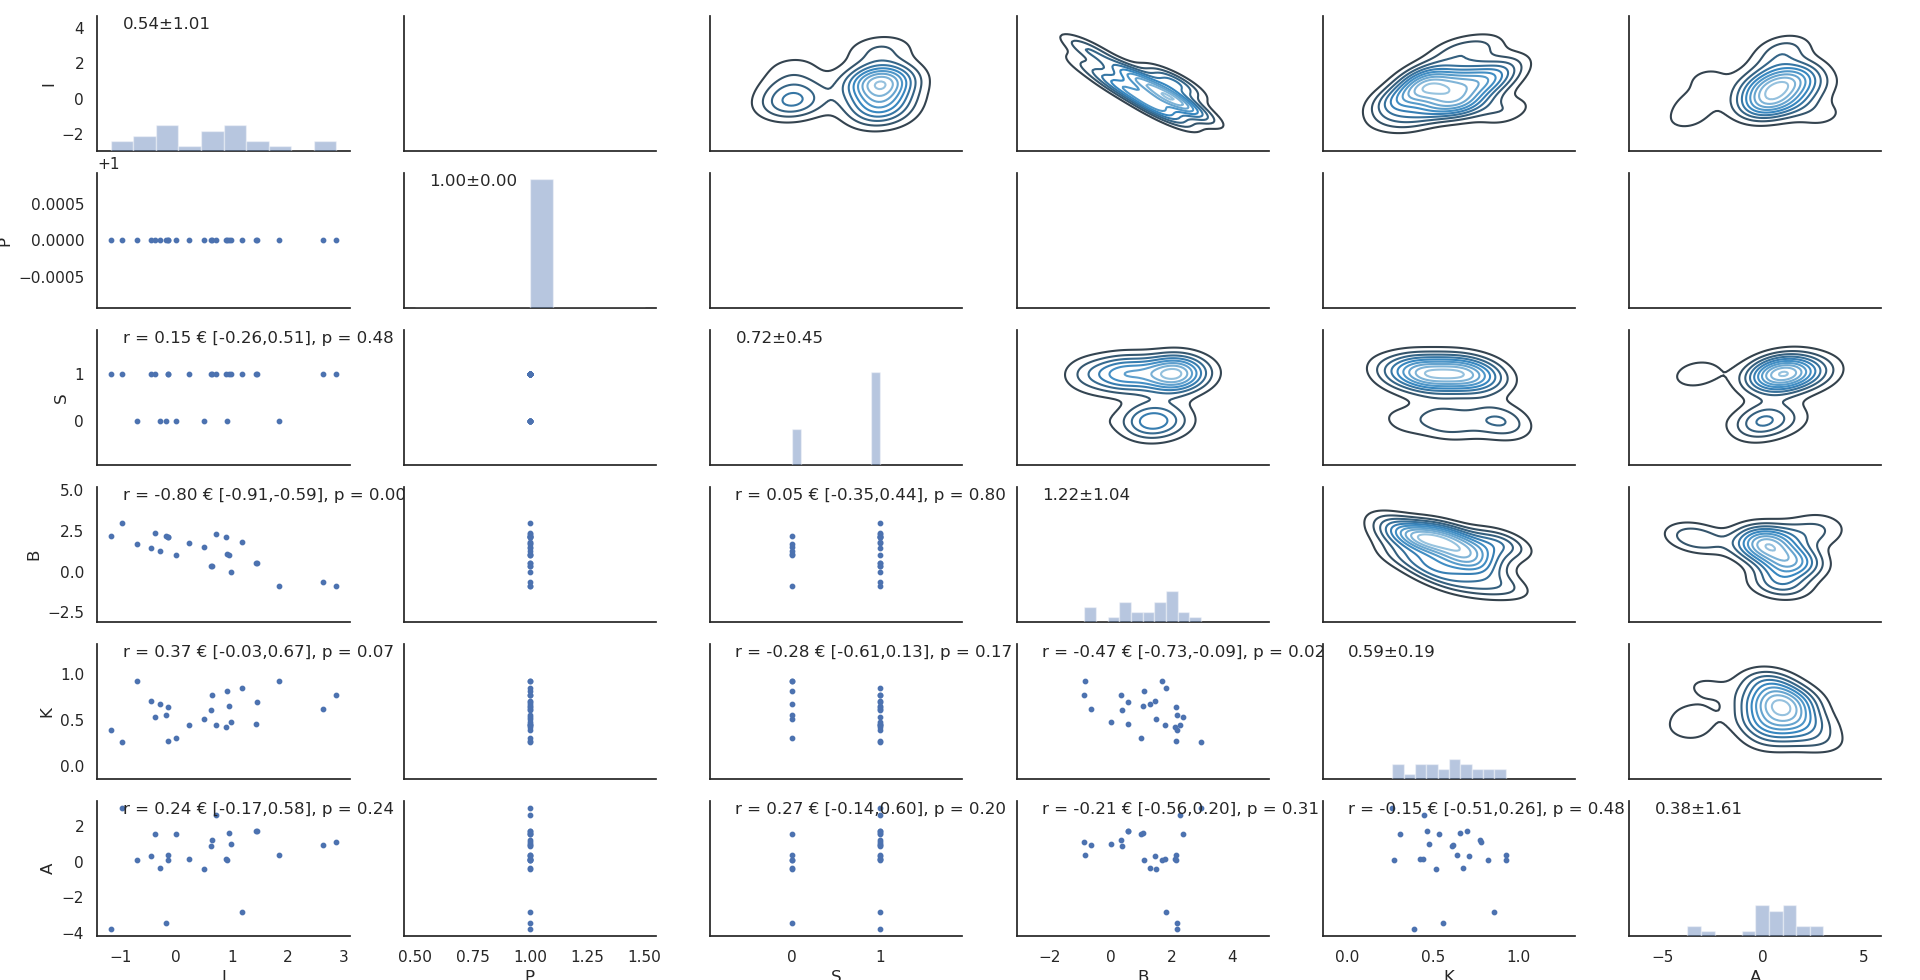
\includegraphics[width=\linewidth]{interPdata}
	\caption{Visualization of the data set under P intervened to 1}
	\label{fig:interPdata}
\end{figure}
\begin{figure}[H]
	\centering
	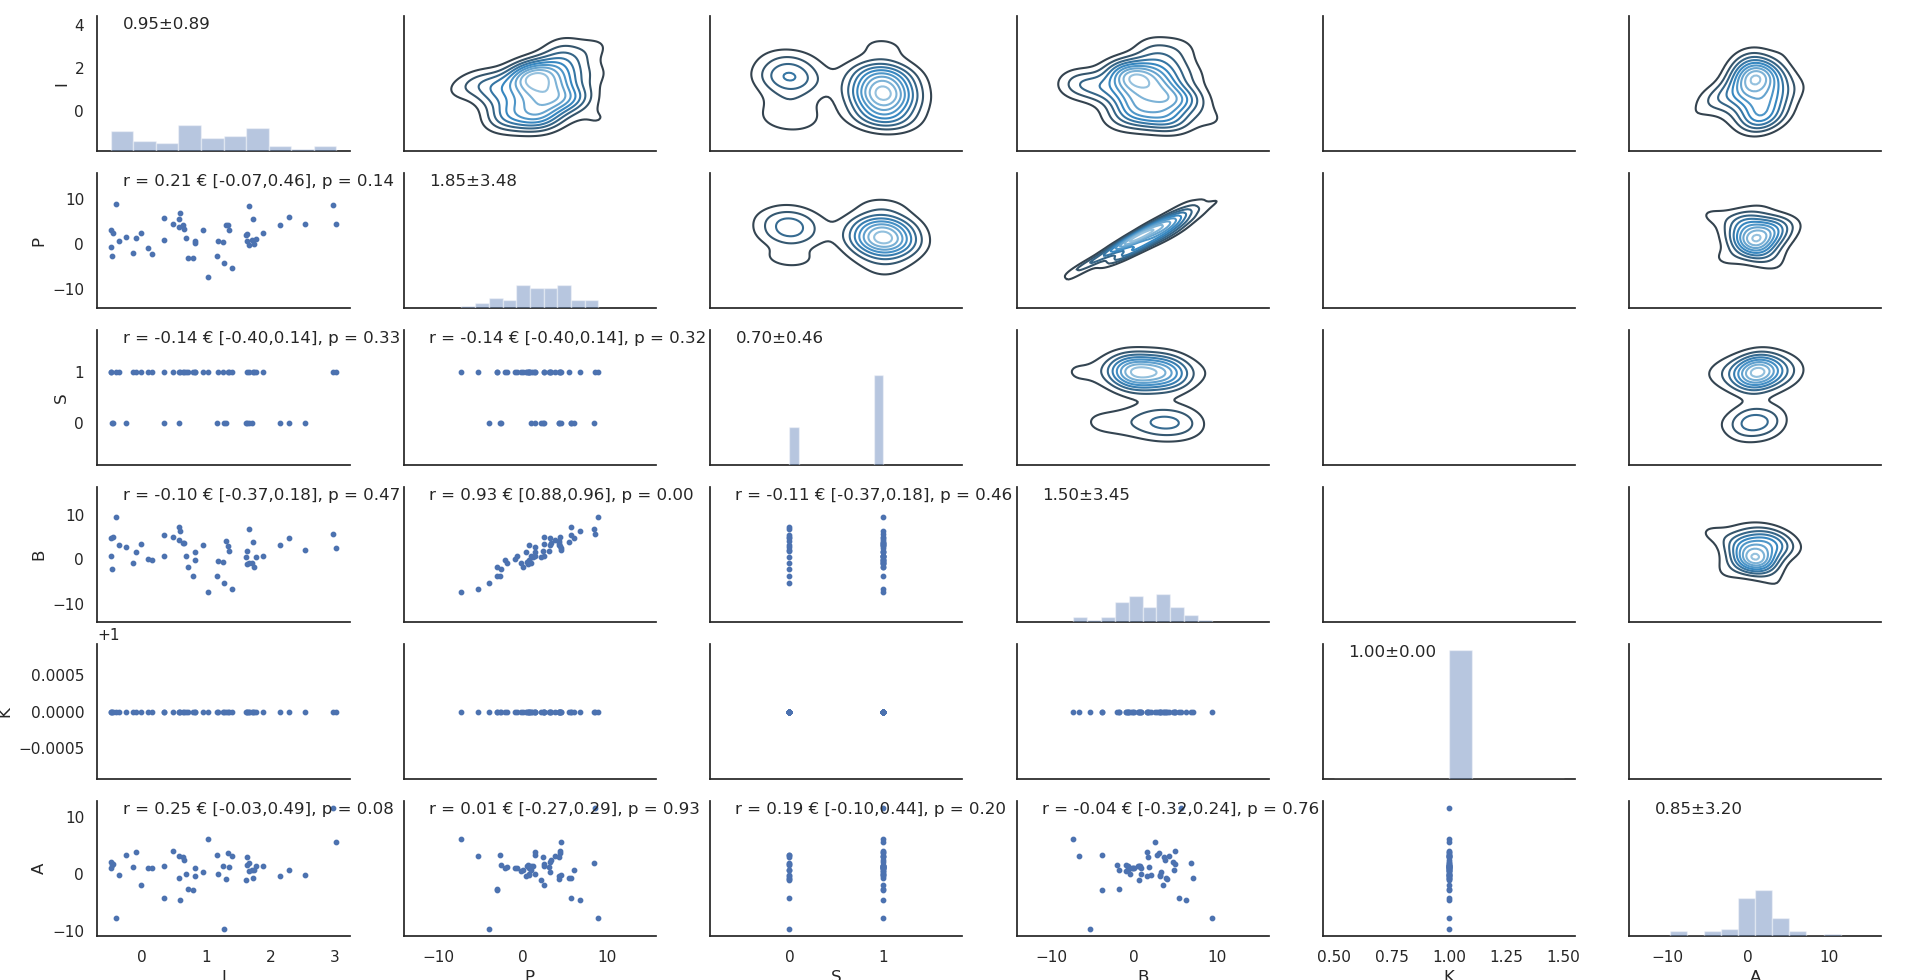
\includegraphics[width=\linewidth]{interKdata}
	\caption{Visualization of the data set under K intervened to 1}
	\label{fig:interKdata}
\end{figure}
\begin{figure}[H]
	\centering
	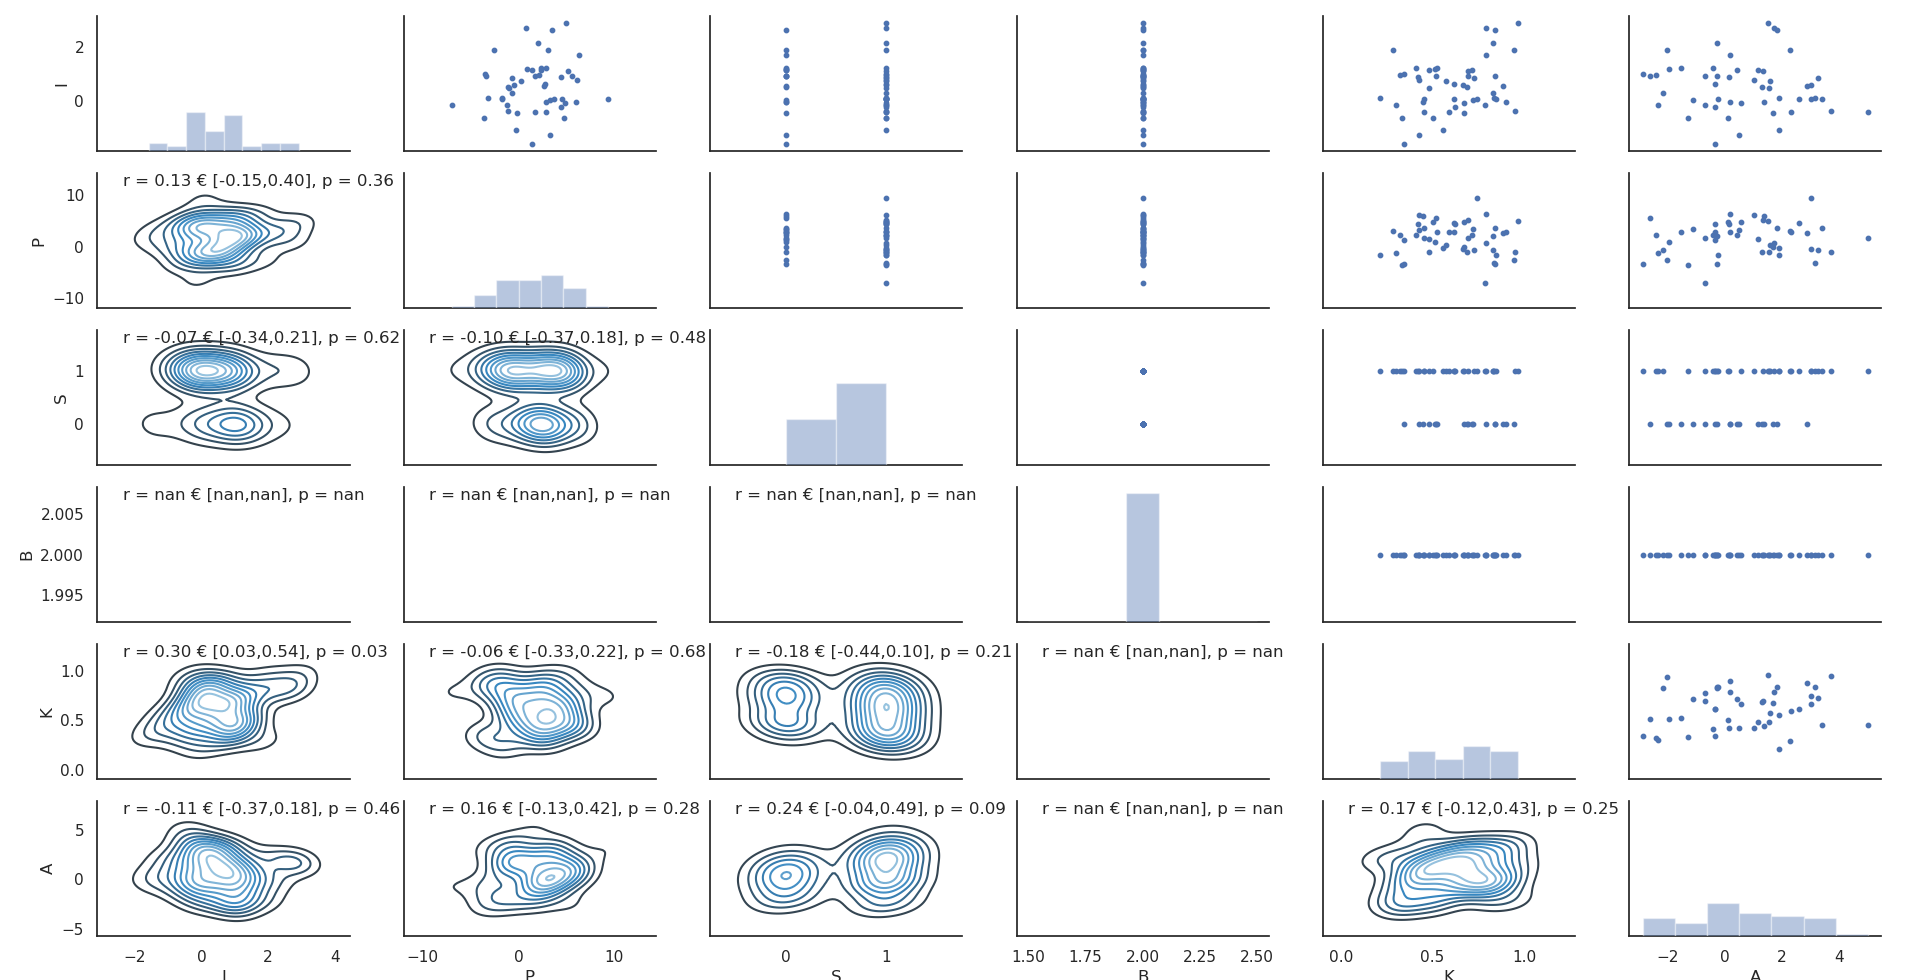
\includegraphics[width=\linewidth]{interBdata}
	\caption{Visualization of the data set under B intervened to 1}
	\label{fig:interBdata}
\end{figure}
\begin{figure}[H]
	\centering
	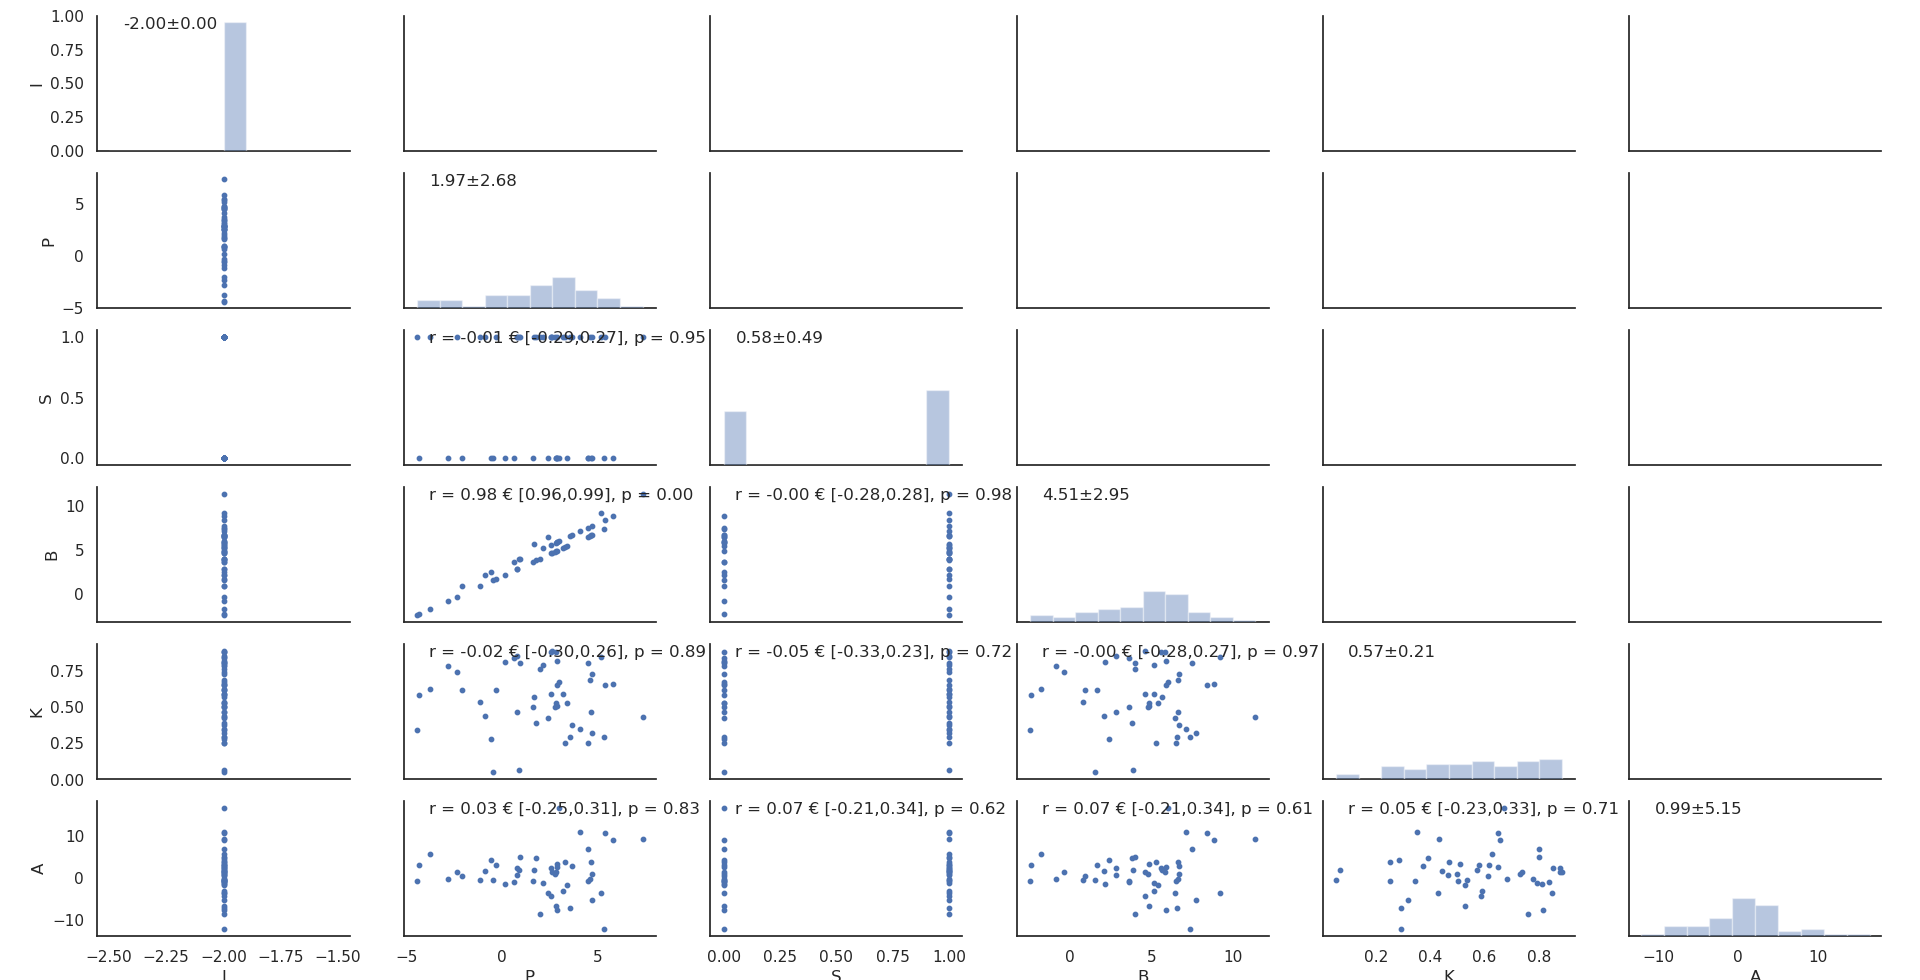
\includegraphics[width=\linewidth]{interIdata}
	\caption{Visualization of the data set under I intervened to -2}
	\label{fig:interIdata}
\end{figure}
\begin{figure}[H]
	\centering
	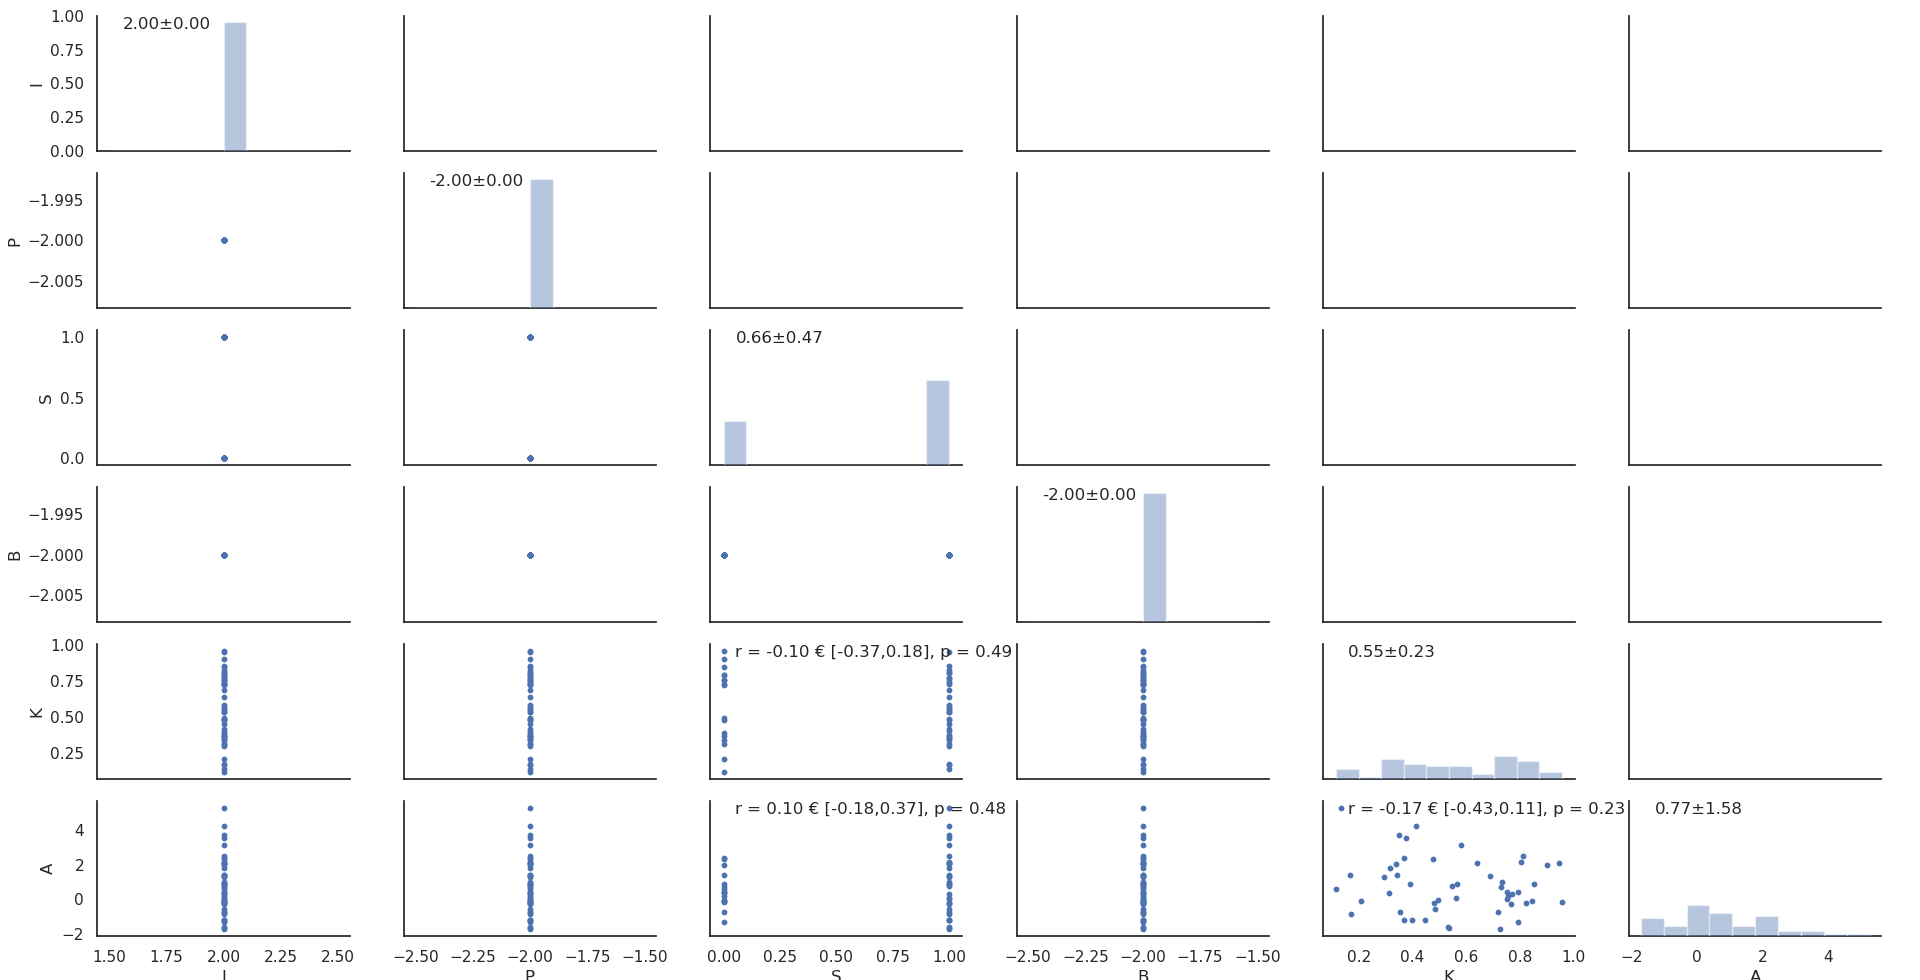
\includegraphics[width=\linewidth]{interIPBdata}
	\caption{Visualization of the data set under I intervened to 2, P to -2 and B to -2}
	\label{fig:interIPBdata}
\end{figure}
\begin{figure}[H]
	\centering
	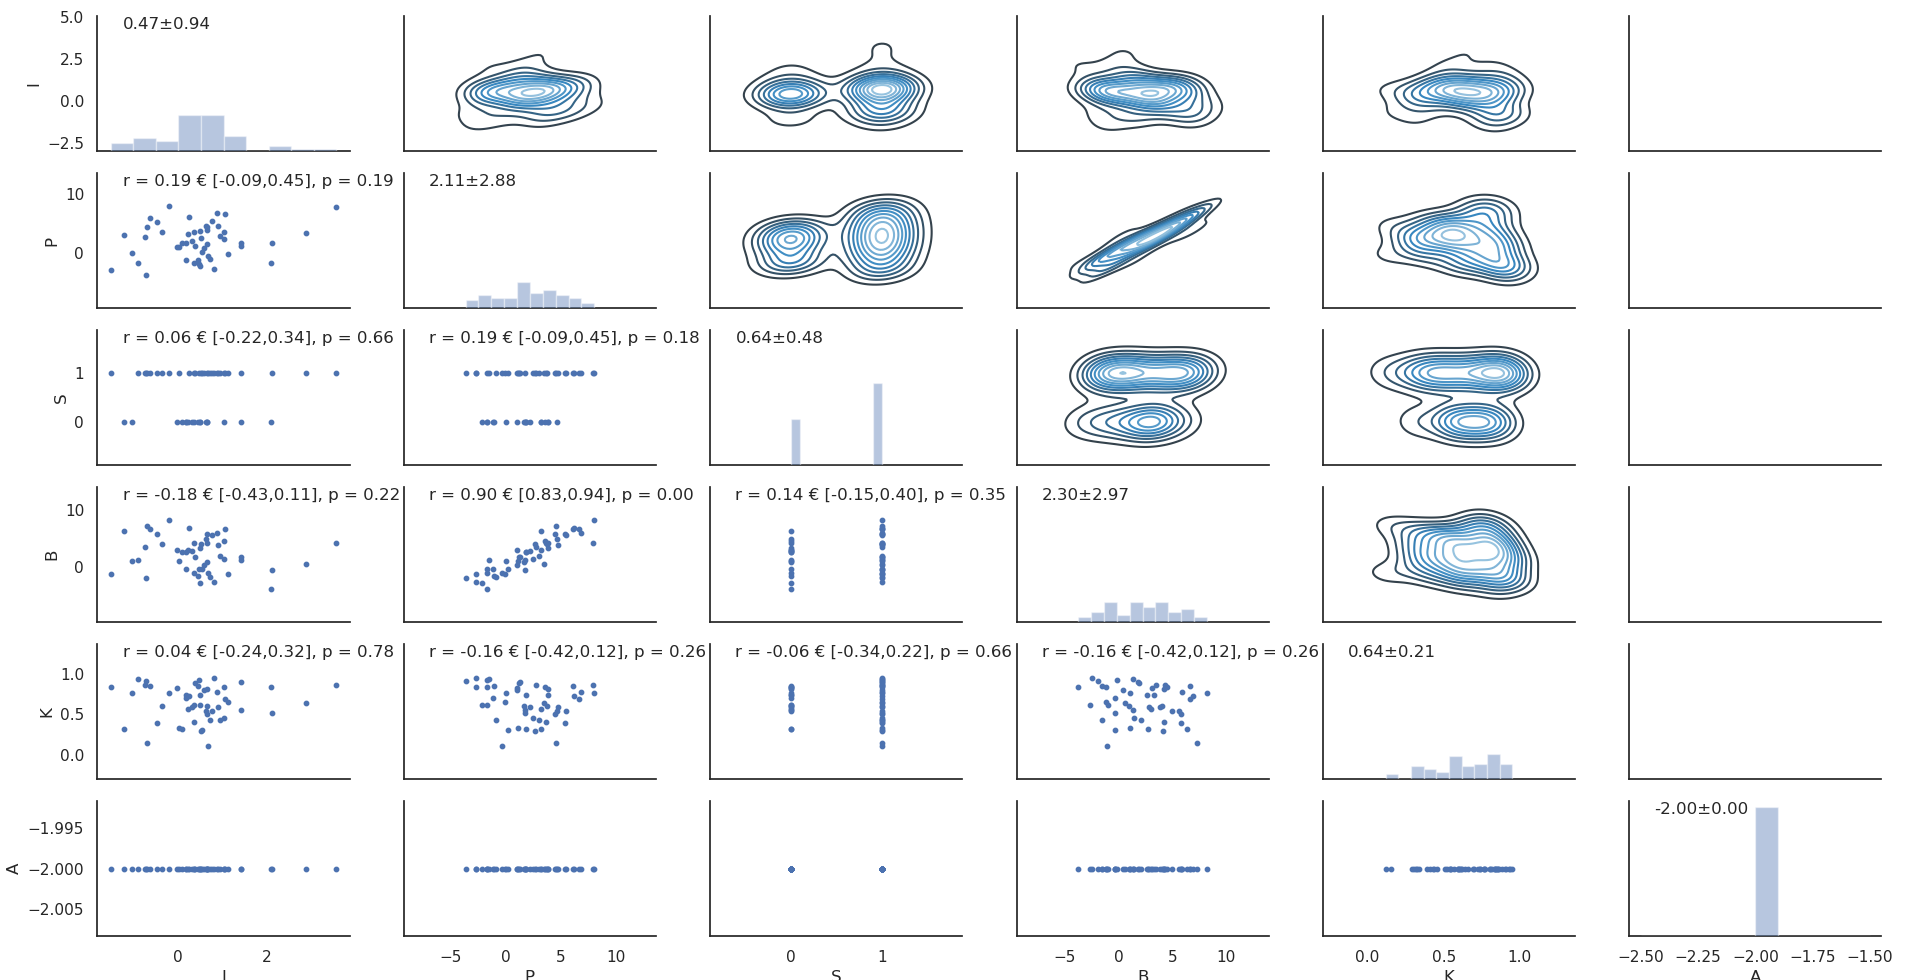
\includegraphics[width=\linewidth]{interAdata}
	\caption{Visualization of the data set under A intervened to -1}
	\label{fig:interAdata}
\end{figure}
\begin{figure}[H]
	\centering
	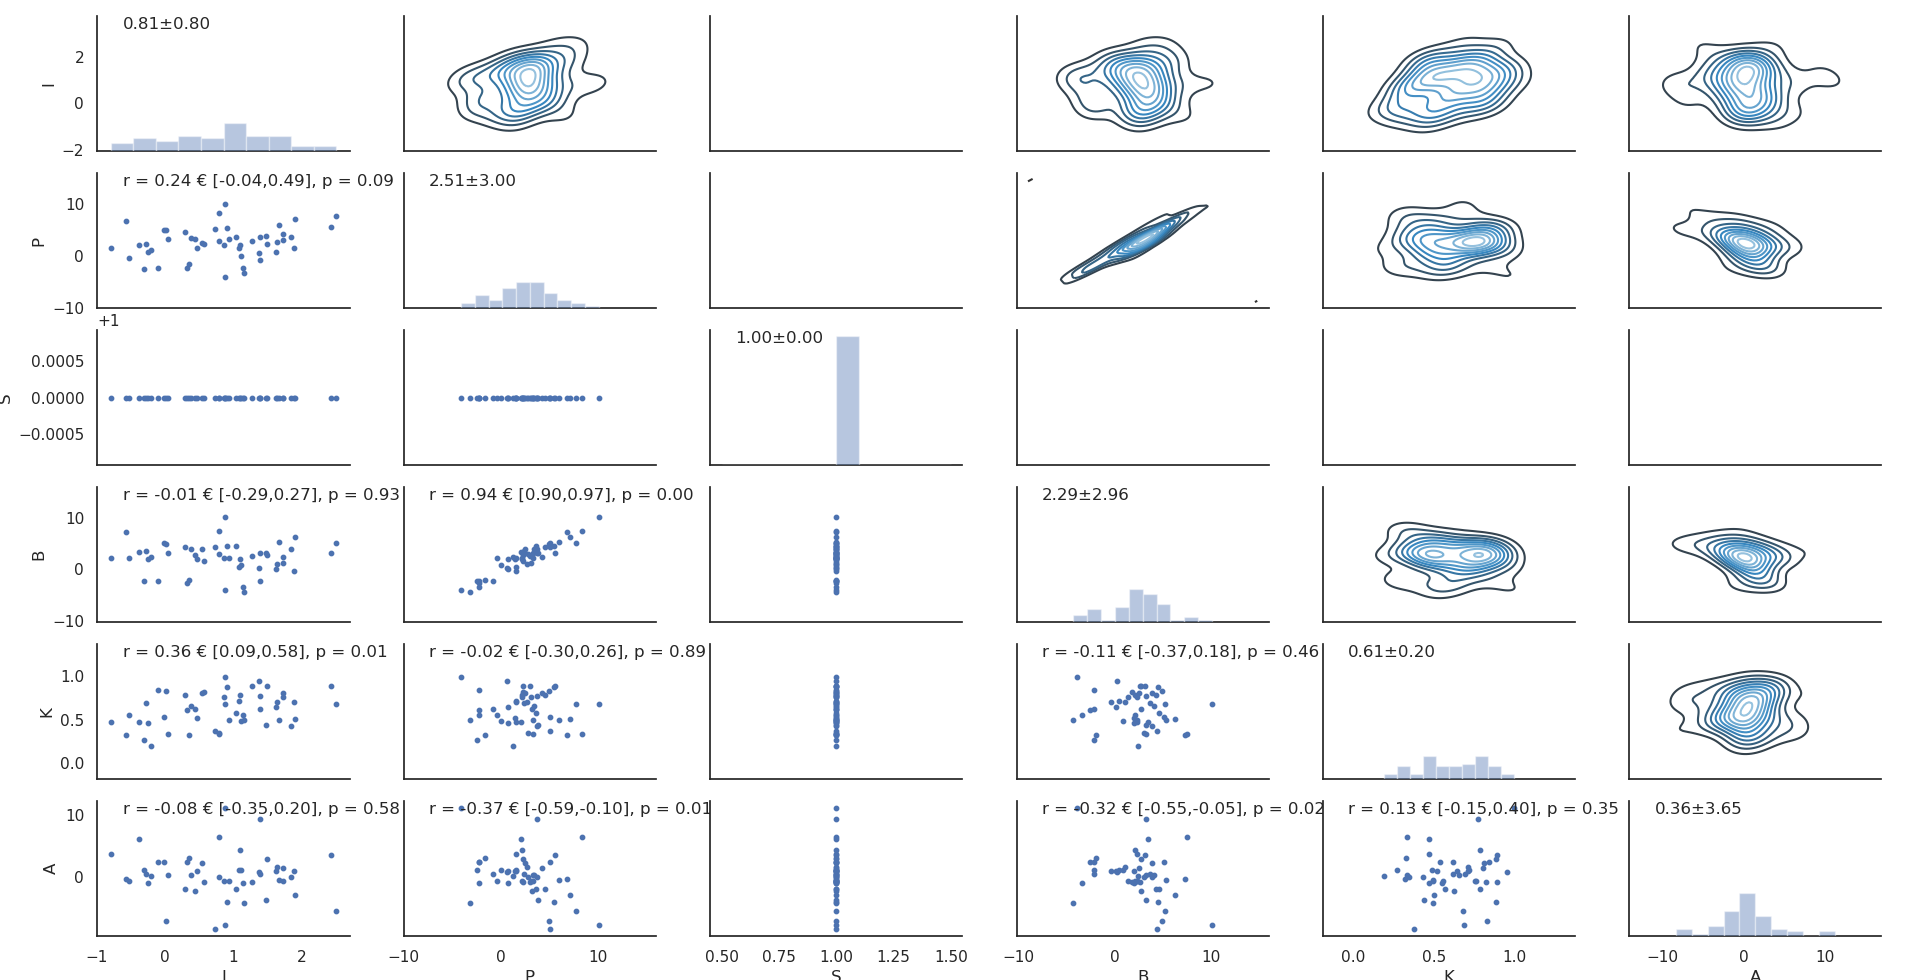
\includegraphics[width=\linewidth]{interSdata}
	\caption{Visualization of the data set under S intervened to 1}
	\label{fig:interSdata}
\end{figure}
\begin{figure}[H]
	\centering
	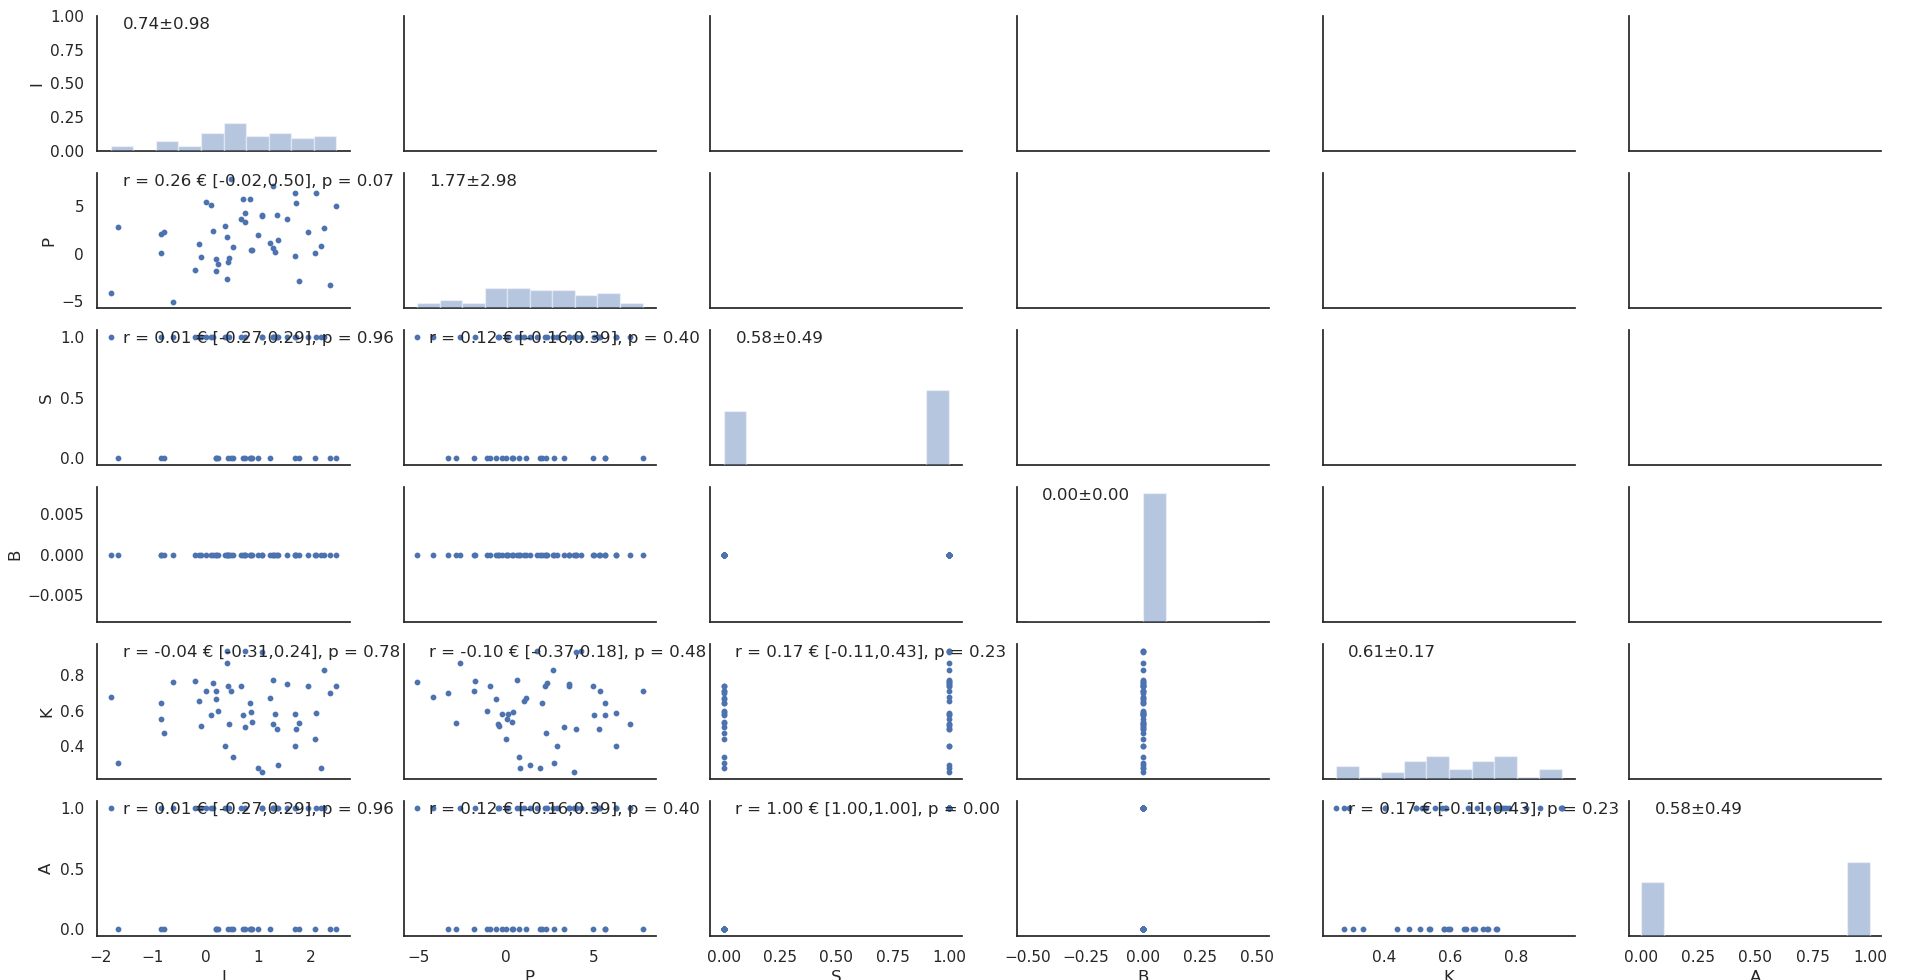
\includegraphics[width=\linewidth]{interB0data}
	\caption{Visualization of the data set under B intervened to 0. }
	\label{fig:interB0data}
\end{figure}

\end{document}

















